\stepcounter{mysection}\section{\arabic{mysection} Сравнительный анализ}

	Как было упомянуто выше одним из основных критериев является средняя длительность ожиданий.
		Так же можно сравнить время выполнения модуляции, объём занимаемой памяти и сложность реализации.
		Под сложностью мы будем понимать суммарное количество строк кода каждого из проектов.

	Сравнив были получены следующие данные.

		Среднее время ожидания:
			\begin{figure}[!htb]
					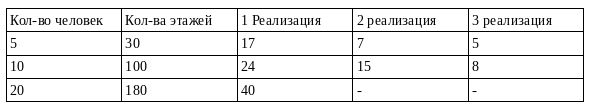
\includegraphics[width=\linewidth]{src/1.png}
					\centering
			\end{figure}

		Реальное время выполнения модуляции:
			\begin{figure}[!htb]
					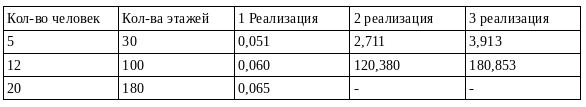
\includegraphics[width=\linewidth]{src/2.png}
					\centering
			\end{figure}

		Объём и сложность:
			\begin{figure}[!htb]
					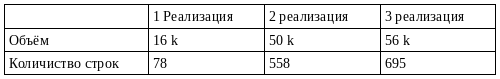
\includegraphics[width=\linewidth]{src/3.png}
					\centering
			\end{figure}

		Входе выполнения экспериментов на выполнение модуляций с большими числами не хватило вычислительной мощи
		оборудования для реализаций на Prolog. Что иллюстрирует потребность в ресурсах у данных подходов
		к решению задачи.

		Но не смотря на провал с большими числами. Третья реализация показала себя лучше, чем остальные.
